\documentclass[tikz,border=3pt]{standalone}
\usepackage{newtxtext,newtxmath}
\usepackage{tikz}
\usetikzlibrary{arrows.meta,positioning,fit,calc,backgrounds}

\definecolor{cproc}{HTML}{4477AA}   % processed / model / legit (blue)
\definecolor{cdead}{HTML}{777777}   % out-of-window / dead (gray)
\definecolor{catk}{HTML}{CC3311}    % attack (red)
\definecolor{cover}{HTML}{EE7733}   % conflation / self-conditioning (orange)
\definecolor{cok}{HTML}{117733}     % propagation-only (green)

\begin{document}
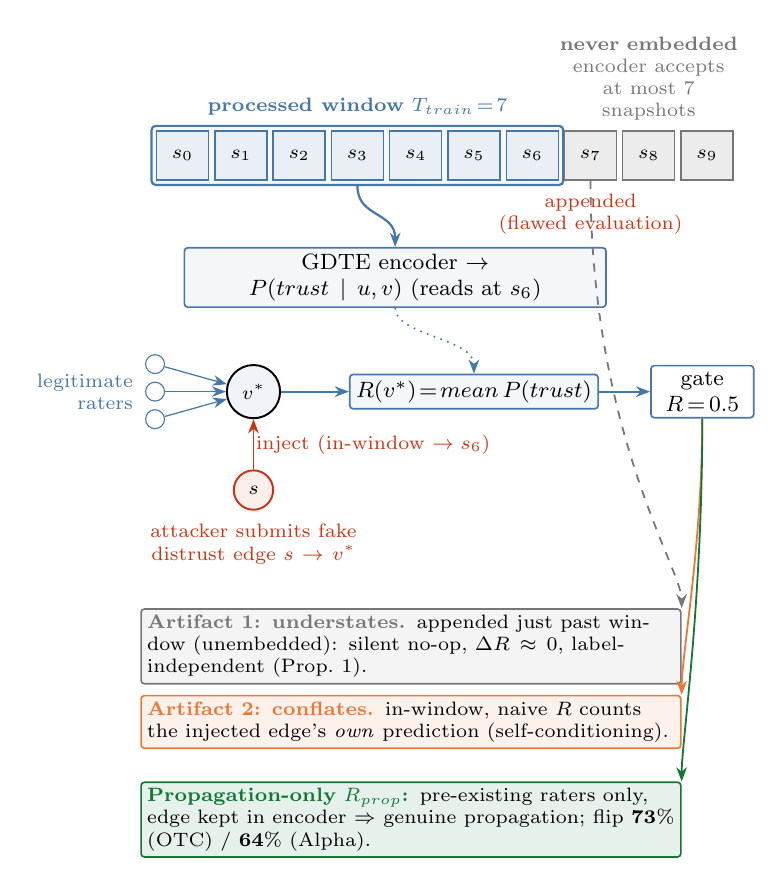
\begin{tikzpicture}[
  font=\footnotesize,
  >={Stealth[length=1.8mm]},
  box/.style={draw,rounded corners=1.2pt,align=center,inner sep=2.2pt,line width=0.6pt},
  snap/.style={draw,minimum width=6.6mm,minimum height=6.2mm,inner sep=0pt,font=\scriptsize,line width=0.5pt},
  proc/.style={snap,draw=cproc,fill=cproc!12},
  dead/.style={snap,draw=cdead,fill=cdead!14},
  lbl/.style={font=\scriptsize,align=center},
  flow/.style={->,line width=0.8pt,draw=cproc},
  ob/.style={box,text width=6.7cm,align=left,font=\scriptsize},
]

% ============ TIMELINE ============
\foreach \i in {0,...,6}{\node[proc] (s\i) at (\i*0.74,0) {$s_{\i}$};}
\foreach \i in {7,8,9}{\node[dead] (s\i) at (\i*0.74,0) {$s_{\i}$};}
\begin{scope}[on background layer]
  \node[draw=cproc,line width=0.8pt,rounded corners=1.5pt,fill=cproc!5,fit=(s0)(s6),inner sep=1.6pt](pwin){};
\end{scope}
\node[lbl,cproc,anchor=south] at (pwin.north){\textbf{processed window} $T_{\text{train}}\!=\!7$};
\node[lbl,cdead,anchor=south,text width=2.4cm] at (s8.north){\textbf{never embedded}\\{\scriptsize encoder accepts\\at most $7$ snapshots}};
\node[catk,font=\scriptsize,align=center,below=0.5mm of s7]{appended\\(flawed evaluation)};

% ============ ENCODER ============
\node[box,draw=cproc,fill=cproc!6,text width=5.2cm] (enc) at (2.7,-1.55)
  {GDTE encoder $\to$ $P(\text{trust}\!\mid\! u,v)$ (reads at $s_6$)};
\draw[flow] (pwin.south)..controls +(0,-0.4) and +(0,0.45)..(enc.north);

% ============ REPUTATION ============
\node[circle,draw,line width=0.7pt,minimum size=5.5mm,fill=cproc!8,font=\scriptsize] (target) at (0.9,-3.0) {$v^\ast$};
\foreach \a/\y in {1/-2.65,2/-3.0,3/-3.35}{
  \node[circle,draw=cproc,line width=0.4pt,minimum size=2.4mm,inner sep=0pt] (r\a) at (-0.35,\y){};
  \draw[->,line width=0.45pt,draw=cproc](r\a)--(target);}
\node[lbl,cproc,left=0.3mm of r2,font=\scriptsize,align=right]{legitimate\\raters};
\node[box,draw=cproc,fill=cproc!6,text width=3.0cm] (rep) at (3.7,-3.0)
  {$R(v^\ast)\!=\!\text{mean}\,P(\text{trust})$};
\node[box,draw=cproc,text width=1.15cm] (gate) at (6.6,-3.0){gate\\$R\!=\!0.5$};
\draw[flow](target)--(rep); \draw[flow](rep)--(gate);
\draw[->,line width=0.6pt,draw=cproc,dotted](enc.south)..controls +(0,-0.35) and +(0,0.45)..(rep.north);

% ============ ATTACK ============
\node[circle,draw=catk,line width=0.7pt,minimum size=4.6mm,fill=catk!8,font=\scriptsize] (atk) at (0.9,-4.25){$s$};
\node[lbl,catk,below=0.5mm of atk,font=\scriptsize,align=center,text width=3.6cm]{attacker submits fake distrust edge $s\!\to\!v^\ast$};
\draw[->,line width=0.7pt,draw=catk](atk)--node[right,catk,font=\scriptsize,inner sep=0.6pt]{inject (in-window $\to s_6$)}(target);

% ============ THREE OUTCOMES (stacked) ============
\node[ob,draw=cdead,fill=cdead!8,anchor=north] (a1) at (2.9,-5.75)
  {\textbf{\textcolor{cdead}{Artifact 1: understates.}} appended just past window (unembedded): silent no-op, $\Delta R\!\approx\!0$, label-independent (Prop.~1).};
\node[ob,draw=cover,fill=cover!10,anchor=north] (a2) at (2.9,-6.85)
  {\textbf{\textcolor{cover}{Artifact 2: conflates.}} in-window, naive $R$ counts the injected edge's \emph{own} prediction (self-conditioning).};
\node[ob,draw=cok,fill=cok!10,anchor=north] (ok) at (2.9,-7.95)
  {\textbf{\textcolor{cok}{Propagation-only $R_{\text{prop}}$:}} pre-existing raters only, edge kept in encoder $\Rightarrow$ genuine propagation; flip $\mathbf{73\%}$ (OTC) / $\mathbf{64\%}$ (Alpha).};

\draw[->,line width=0.65pt,draw=cdead,dashed] (s7.south)..controls +(0,-3.2) and +(0,0.5)..(a1.north east);
\draw[->,line width=0.65pt,draw=cover] (gate.south)..controls +(0,-1.6) and +(0,0.5)..(a2.north east);
\draw[->,line width=0.65pt,draw=cok] (gate.south)..controls +(0,-2.4) and +(0,0.5)..(ok.north east);

\end{tikzpicture}
\end{document}
